\section{Project methodology}
\label{sec:proj-meth}
In this section the project methodologies tools are outlined, easing the
development process.

\subsection{Waterfall model}
\label{sec:waterfall-model}
For the domain-specific design of software the waterfall methodology is used.
The waterfall model (fig.~\ref{fig:waterfall}) represents the first effort to
conveniently tackle the increasing complexity in the software development
process, being credited to Royce, in 1970, the first formal description of the
model, even though he did not coin the term~\cite{sommerville1996software}. It
envisions the optimal method
as a linear sequence of phases, starting from requirement elicitation to system
testing and product shipment~\cite{cusumano1995beyond} with the process flowing
from the top to the bottom, like a cascading waterfall.

In general, the phase sequence is as follows: analysis, design, implementation,
verification and maintenance.
\begin{enumerate}
  \item Firstly, the project requirements are elicited, identifying the key
    requirements and constraints the system being developed must meet from the
    end-user perspective, captured in natural language in a product requirements document.
  \item In the analysis phase, the developer should convert the application
    level knowledge, enlisted as requirements, to the solution domain knowledge
    resulting in analysis models, schema and business rules.
  \item In the design phase, a thorough specification is written allowing the
    transition to the implementation phase, yielding the decomposition in
    subsystems and the software architecture of the system. 
  \item In the implementation stage, the system is developed, following the
    specification, resulting in the source code.
  \item Next, after system assembly and integration, a verification phase occurs
    and system tests are performed, with the systematic discovery and debugging
    of defects.
  \item Lastly, the system becomes a product and, after deployment, the
    maintenance phase start, during the product life time.
\end{enumerate}
While this cycle occurs, several transitions between multiple phases might
happen, since an incomplete specification or new knowledge about the system,
might result in the need to rethink the document.

The advantages of the waterfall model are: it is simple and easy to understand
and use and the phases do not overlap; they are completed sequentially. However,
it presents some drawbacks namely: difficulty to tackle change and high
complexity and the high amounts of risk and uncertainty. However, in the present
work, due to its simplicity, the waterfall model proves its usefulness and will
be used along the project.

As a reference in the sequence of phases and the expected outcomes from each
one, it will be used the chain of development activities and their products
depicted in fig.~\ref{fig:sw-devel-activities} (withdrawn from
\cite{bruegge2004object}).

\begin{figure}[!hbt]
\centering
    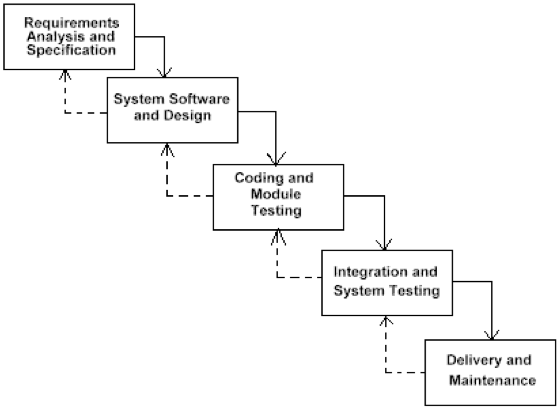
\includegraphics[width=0.6\textwidth]{./img/waterfall.png}
  \caption{Waterfall model diagram}\label{fig:waterfall}
\end{figure}

\subsection{Unified Modeling Language (UML)}
\label{subsec:uml}
To aid the software development process, a notation is required, to articulate
complex ideas succinctly and precisely. The notation chosen was the \gls{uml},
as it provides a spectrum of notations for representing different aspects of a
system and has been accepted as a standard notation in the software
industry~\cite{bruegge2004object}.

The goal of UML is to provide a standard notation that can be used by all
object- oriented methods and to select and integrate the best elements of
precursor software notations, namely \gls{omt}, Booch, and \gls{oose}
~\cite{bruegge2004object}. It provides
constructs for a broad range of systems and activities (e.g., distributed
systems, analysis, system design, deployment). System development focuses on
three different models of the system
(fig.~\ref{fig:sw-devel-activities})~\cite{bruegge2004object}:
\begin{enumerate}
  \item \textbf{\emph{The functional model}}: represented in UML with use case
    diagrams, describes the functionality of the system from the user's point of
    view.
  \item \textbf{\emph{The object model}}: represented in UML with class
    diagrams, describes the structure of the system in terms of objects,
    attributes, associations, and operations.  
  \item \textbf{\emph{The dynamic model}}: represented in UML with interaction
    diagrams, state-machine diagrams, and activity diagrams, describes the
    internal behaviour of the system.
\end{enumerate}

\begin{figure}[!hbt]
\centering
    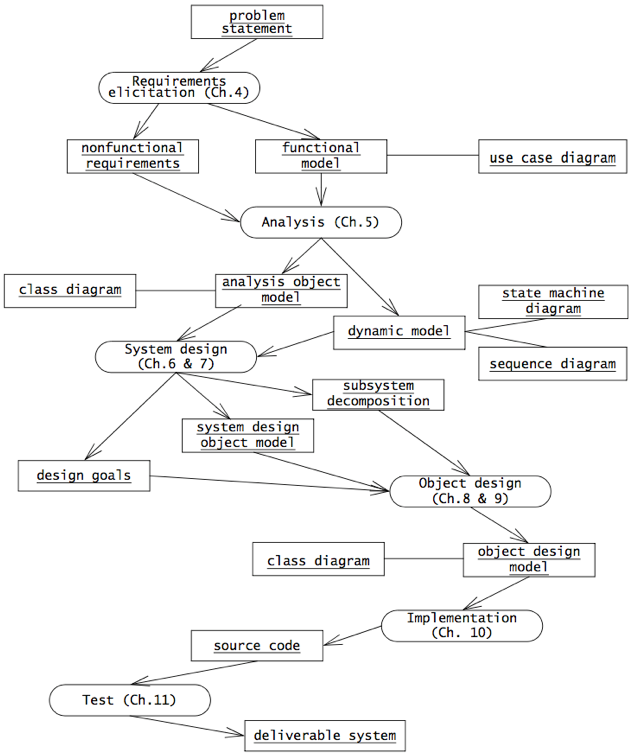
\includegraphics[width=0.7\textwidth]{./img/sw-devel-activities.png}
  \caption{An overview of the object-oriented software engineering development
  and their products. This diagram depicts only logical dependencies among work
  products (withdrawn from~\cite{bruegge2004object})}
\label{fig:sw-devel-activities}
\end{figure}

%%% Local Variables:
%%% mode: latex
%%% TeX-master: "../../../dissertation"
%%% End:
